\section{Experimental validation}
Tests are executed on the Intel Xeon Phi KNC, with 64 physical cores with a four-way multithread support each, for a total of 256 threads.

For the text we have prepared an \textit{auto} mode that automatically runs the benchmarks for the provided input values. It runs the sequential, parallel and fastflow version, and for the latter two runs test with an increasing number of workers. At the end of the execution, the automatic mode provides a summary of the timestamps, in addition to those printed during the execution.

The time of each test is expressed in millisecond. Each timestamp provided in this document represent the averages of the timestamps of 5 tests performed with the same parameters.



\subsection{Sequential algorithm}
The sequential version with a window size $w = 100$, a tuple size $t = 10$, a sliding factor $k = 1$ and a stream length $l = 100000$ takes $\sim 24000 \ msec$ on the Intel Xeon Phi.

\bigskip\noindent
We also computed the partial times, measuring the time spent in the single operations with this parameter. We implemented the print as a delete of the skyline, since the actual print on standard out or file takes a very long time and is not scalable, hence we found it less interesting to be considered.

\medskip\noindent
Pick the windows from the stream: $\sim 88 \ msec$, i.e. $\sim 0.88 \ \mu sec$ each, i.e. $\sim 0,36\%$.\\
Process the windows: $\sim 24000 \ msec$, i.e. $\sim 240 \ \mu sec$ each, i.e. $\sim 99,39\%$.\\
Delete the skylines: $\sim 60 \ msec$, i.e. $\sim 0.6 \ \mu sec$ each, i.e. $\sim 0,25\%$.\\

\bigskip\noindent
Process a window takes $\sim 272$ times the time to pick it and $\sim 400$ times the time needed to delete the corresponding skyline. Since the Intel Xeon Phi supports up to 256 cores, we should be able to sped up the application by scaling on the second step, i.e. the computation of the skyline.



\subsection{Completion times}
\begin{table}[H]
    \centering
    \begin{tabular}{|l|c|r|r|r|r|r|}
\hline
           & nw  & w = 128 & w = 256  & w = 512  & w = 1024  & w = 2048  \\ \hline
Sequential & 1   & 4970262 & 18585713 & 68950202 & 258524148 & 897301533 \\ \hline
Parallel   & 1   & 5343199 & 19621995 & 70448451 & 257031126 & 898974927 \\ \hline
Parallel   & 2   & 2680228 & 9903538  & 36605589 & 134886437 & 475516158 \\ \hline
Parallel   & 4   & 1334705 & 4939809  & 18432914 & 67388771  & 237680980 \\ \hline
Parallel   & 8   & 668252  & 2480417  & 9186436  & 33835748  & 120349829 \\ \hline
Parallel   & 16  & 344069  & 1244297  & 4591405  & 16792859  & 59501326  \\ \hline
Parallel   & 32  & 199679  & 632766   & 2307841  & 8501624   & 30764311  \\ \hline
Parallel   & 64  & 119624  & 405146   & 1362731  & 4413848   & 15859510  \\ \hline
Parallel   & 128 & 193414  & 290523   & 950836   & 3220670   & 11374157  \\ \hline
Parallel   & 256 & 200697  & 246579   & 797835   & 2700211   & 9327988   \\ \hline
Fastflow   & 1   & 5279013 & 19650859 & 72988778 & 267977425 & 952241207 \\ \hline
Fastflow   & 2   & 2654387 & 9842083  & 36545246 & 134163459 & 475243530 \\ \hline
Fastflow   & 4   & 1331611 & 4940133  & 18263974 & 67077633  & 237621958 \\ \hline
Fastflow   & 8   & 671599  & 2481758  & 9156595  & 33563912  & 118830059 \\ \hline
Fastflow   & 16  & 342098  & 1242880  & 4613028  & 16901159  & 59797504  \\ \hline
Fastflow   & 32  & 200525  & 637487   & 2340830  & 8449103   & 30362855  \\ \hline
Fastflow   & 64  & 168367  & 557349   & 2012049  & 7253576   & 25046960  \\ \hline
Fastflow   & 128 & 149153  & 443139   & 1488754  & 5066831   & 17368437  \\ \hline
Fastflow   & 256 & 478662  & 670081   & 1209638  & 3929258   & 13397304  \\ \hline
\end{tabular}
    \bigskip
    \captionof{table}{Completion times}
\end{table}



\subsection{Speedup}
\begin{figure}[H]
    \centering
    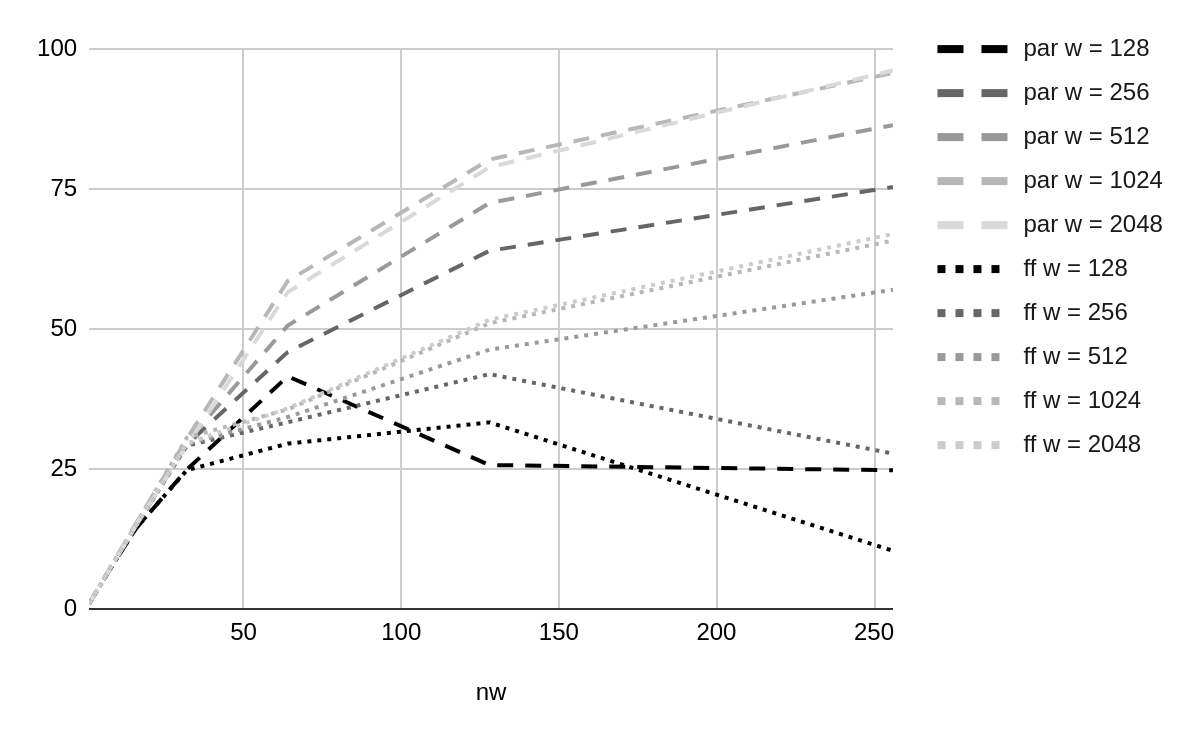
\includegraphics[width=\linewidth]{assets/speedup}
    \bigskip
    \captionof{figure}{Speedup chart}
\end{figure}



\subsection{Scalability}
\begin{figure}[H]
    \centering
    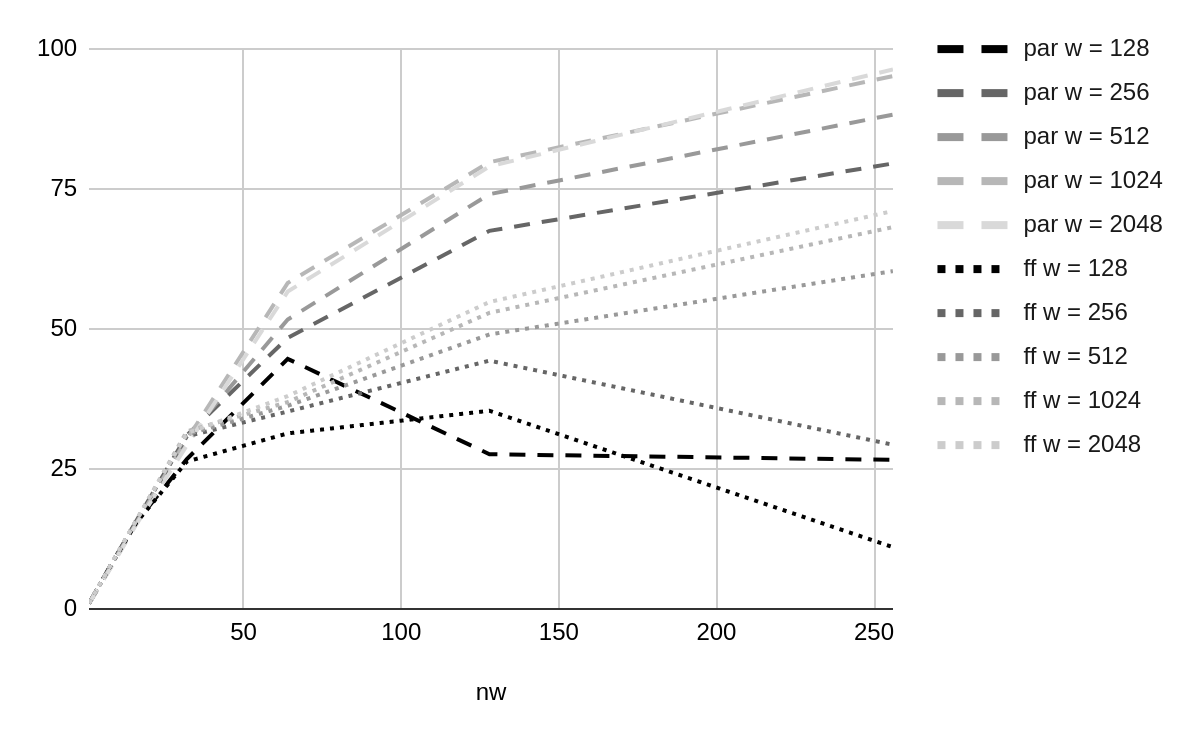
\includegraphics[width=\linewidth]{assets/scalability}
    \bigskip
    \captionof{figure}{Scalability chart}
\end{figure}



\subsection{Efficiency}
\begin{figure}[H]
    \centering
    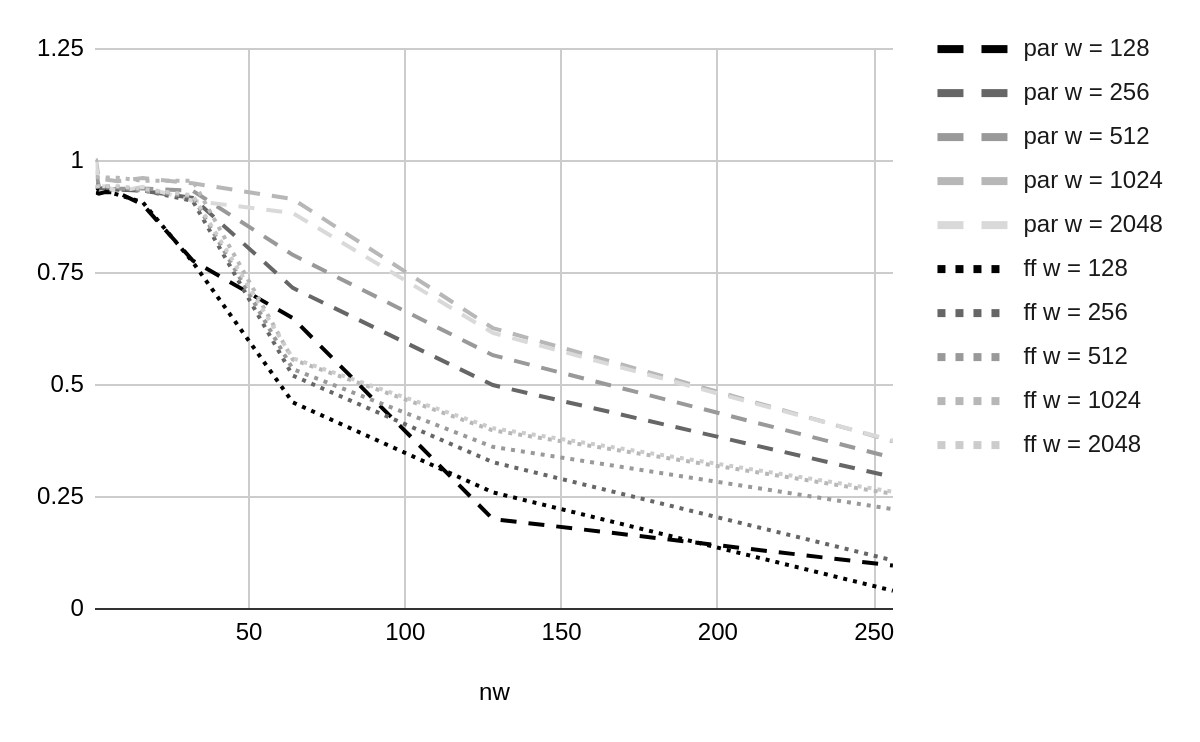
\includegraphics[width=\linewidth]{assets/efficiency}
    \bigskip
    \captionof{figure}{Efficiency chart}
\end{figure}